%This file will be included in the ThesisMain Document as the experimentation
%section.

%Author: James Kelly
%Last Modified: 11-12-08

\begin{center}
\section{Theory}
\end{center}

The data from the stormwater discharge simulation trials support several elementary theories that successfully model and predict energy transfer outcomes. These concepts and models can in all likelihood be applied to any unconsolidated material in a gravitationally charged flow scenario. Two separate approaches yield similar outcomes that are aligned with experimental results. Each approach offers the benefit of different conceptualizations and different complexities in parametrization. \\

\subsection{Resistor-Capacitor (RC) Circuit Analogy}
The first of these scenarios involves modeling the vessel circuit as an electrical resistor-capacitor circuit. The conceptualization here stems from the analogy of electrical to thermal potential and is useful when considering specific consequences of heat loss. In this case, the applied voltage to the RC element is directly analogous to the difference between the reservoir temperature and the ambient temperature. This quantity is the total thermal potential and drives the transfer of energy between the fluid flow and the aggregate. 

\begin{figure}
\begin{center}
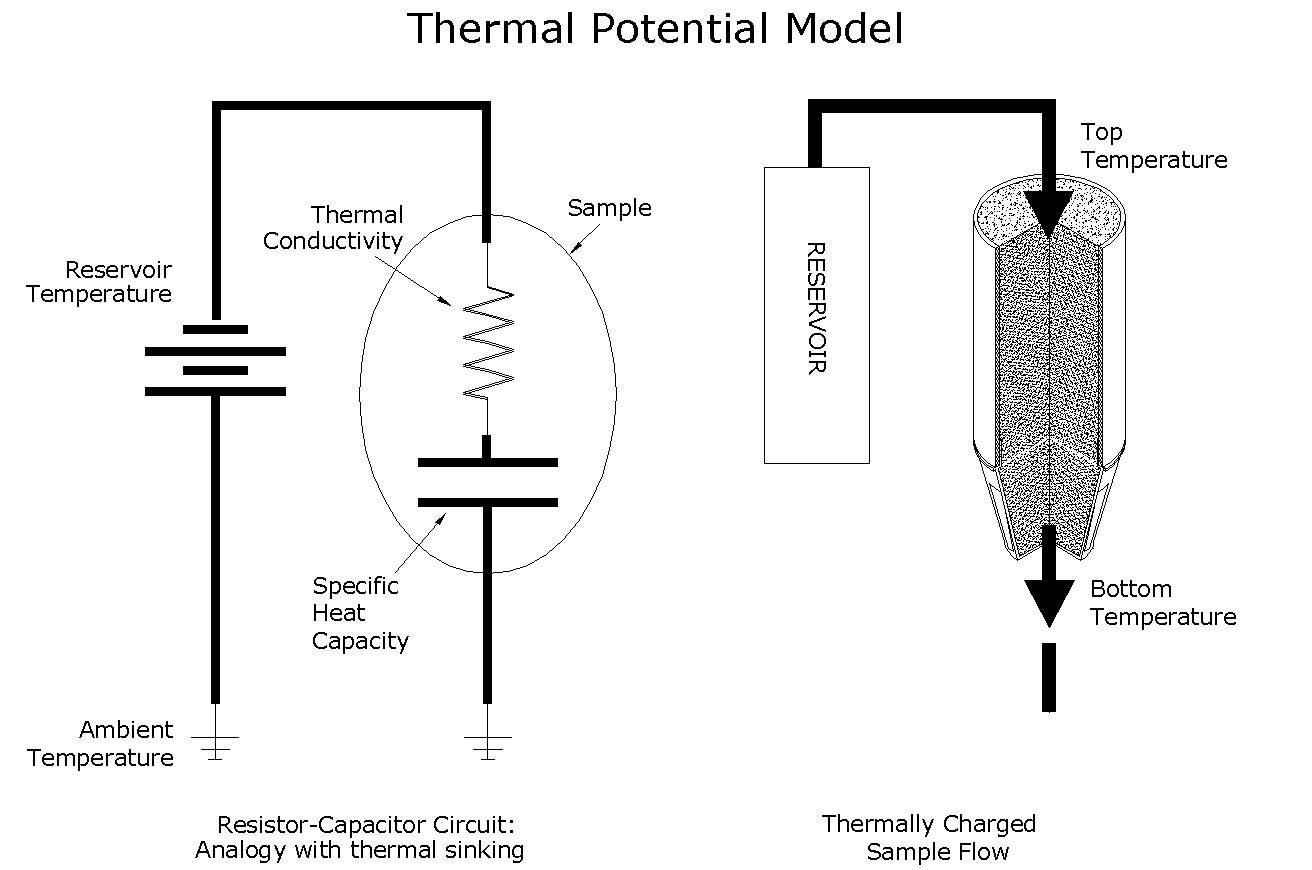
\includegraphics[scale=.35]{RCtherm.jpg}
\caption[Thermal Potential Model]{\textbf{\emph{The Potential Model Analogy}} An RC circuit is shown as a potential model for the sample vessel under thermal load. The net quantity of thermal energy transfered to the thermal sink inside the sample vessel is directly analogous to the capacitance of the RC circuit. The rate of that thermal energy exchange is a function of the thermal conductivity and the temperature difference that drives the exchange. These parameters are analogous to the resistance and applied voltage of the RC circuit.\label{rctherm}}
\end{center}
\end{figure}

Equation \ref{rc} and Figure \ref{rctherm} model the voltage across the capacitor as an RC \linebreak circuit charges \citep{elec}. In upholding the analogy, $V_{C}$ represents the temperature between the aggregate and the fluid flow at a time $t$. 

\begin{equation}\label{rc}
 V_{C}(t)=V(1-e^{\frac{-t}{RC}})
\end{equation}

The second part of this theory section realizes that the temperature gradient between the top and bottom temperature sensors at a time $t$ is not constant or linear, and consequently the temperature between the rock and the fluid will vary not only with time but also with position. Therefore, in applying the RC circuit analogy, $V_{C}$ must be interpreted specifically as the average, bulk temperature difference between fluid and aggregate. Any assumption that the temperture between the top and bottom locations is equivalent to the temperture difference between the water and the rock interface is oversimplified, and so this potential model serves only to describe the thermal sink effects on a bulk scale.

By Equation (\ref{rc}), using $V$ as the total available thermal potential, $T_{o}=T[TOP]-T[AMBIENT]$, substituting the thermal resistivity $\kappa^{-1}$ for $R$, $c_{R}$ as the capacitance $C$ and letting $\sigma$ represent a dimensional constant with units of $\frac{kg}{m}$, a thermal potential equation can be formulated from Equation (\ref{rc}):
\begin{equation}\label{rcNew}
T(t)[R]=T_{o}(1-e^{x})\:\:\:\:\:\:\:x=\frac{\sigma t}{\left[\frac{c_{R}}{\kappa}\right]}
\end{equation}

Figure \ref{rcthyplot} shows the thermal potential model of Equation \ref{rcNew} compared to data for two materials, QM1 and QM6. 

\begin{figure}[h!]

\begin{center}
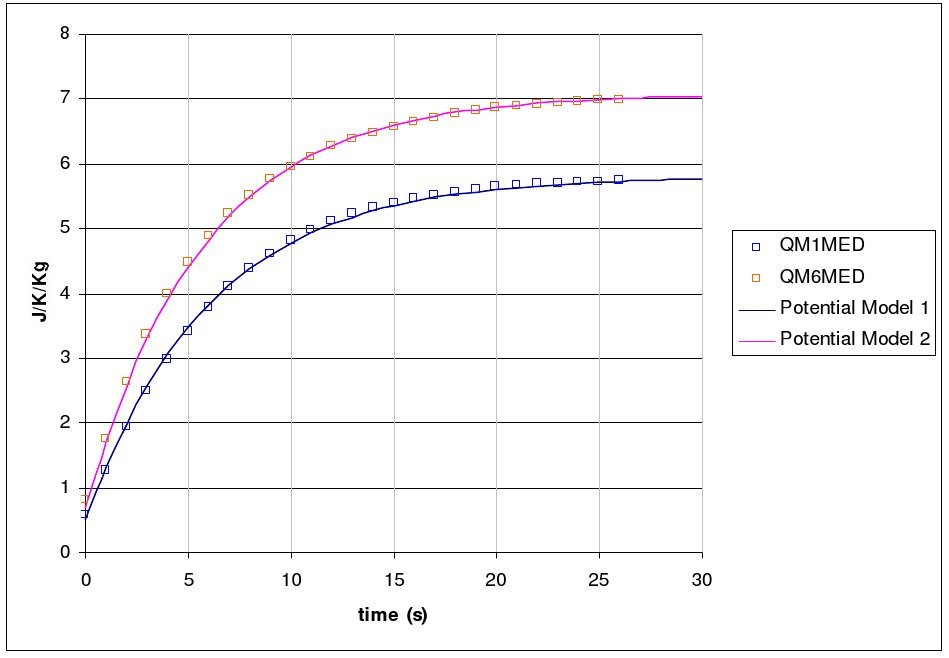
\includegraphics[scale=.4]{rcTheory.jpg}
\caption[Thermal Potential Data Comparison]{\textbf{\emph{A plot of a typical thermal potential model and a typical scaled, normalized CET plot}} Correlation coefficients for both plots was 0.98. Curves were optimized by plotting both dependent variables against one-another in a linear least squares regression model and fitting for a fixed $T_{m}$ value. Only the most extreme aggregate sizes were not well modeled by the thermal potential function, such as QM.3 and QM5 - refer to Figure (\ref{thMom}).\label{rcthyplot}}
\end{center}
\end{figure}

In the analysis of an RC circuit, the time constant $RC$ is used to characterize the response of the RC element. In the analog of that analysis, a new ``time constant'' appears in the exponent and is defined as the \emph{thermal moment}, $T_m$. 

\begin{equation}\label{tm}
T_m\;=\;\dfrac{\kappa}{C_R}
\end{equation}

This thermal moment characterizes how fast and how much heat can be transferred for an available potential, $T_{o}$. Let $\sigma=-\frac{R_{s}}{M_{s}}$ as necessary constants to compliment both $\kappa$ and $C_{R}$ and to dimensionally balance the exponent. 

\begin{equation}\label{rcExp}
x=\frac{\dfrac{R_{s}}{M_{s}} t}{\left[\dfrac{c_{R}}{\kappa}\right]}
\end{equation}

\begin{figure}[h!]
\begin{center}
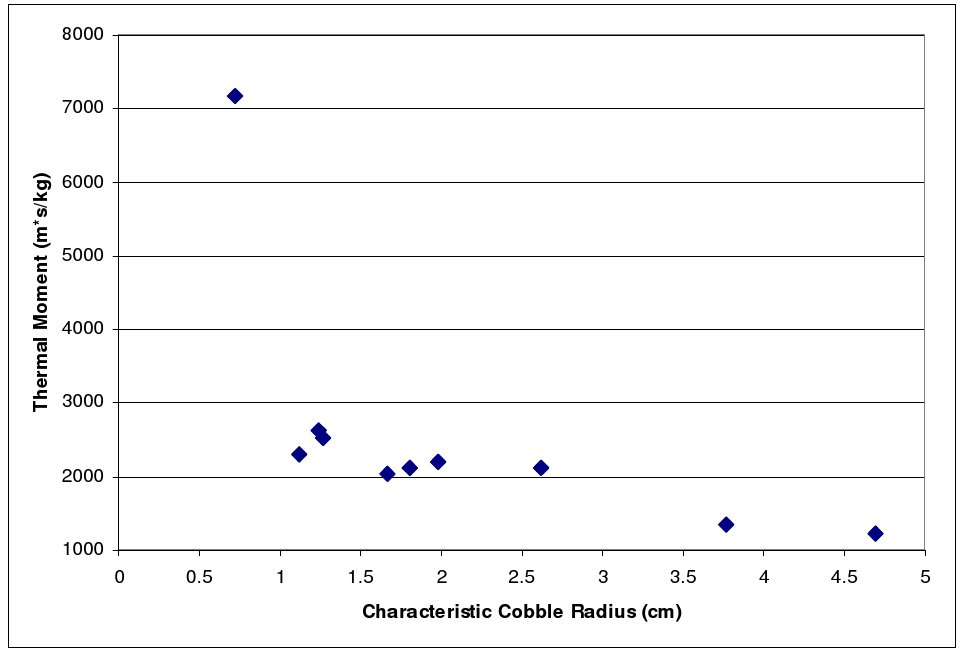
\includegraphics[scale=.4]{thMom.jpg}
\caption[Thermal Moment and Cobble Size]{\textbf{\emph{Thermal Moment and Cobble Size}} This illustrates a result from fitting both medium and low flow trials of the QM samples with Equation (\ref{rcNew}) and then extracting the exponent information to attain a thermal moment.\label{thMom}}
\end{center}
\end{figure}
\pagebreak
This new exponent, expanded in Equation (\ref{rcExp}) is a building block for a more detailed, empirical formulation of the heat exchange process. Unlike the RC circuit model however, flow considerations are taken into account. Additionally, there is one inconsistency of the analogy presented here  in the form of a floating ``boundary'' at the bottom temperature location compared to a grounded or absolute potential with the RC circuit. In the following emipirical formulation, this is taken into account to achieve what looks to be a much more accurate model, albeit with increased complexity.

\subsection{An Empirical Formulation from Experimental Parameters}

\begin{figure}
\begin{center}
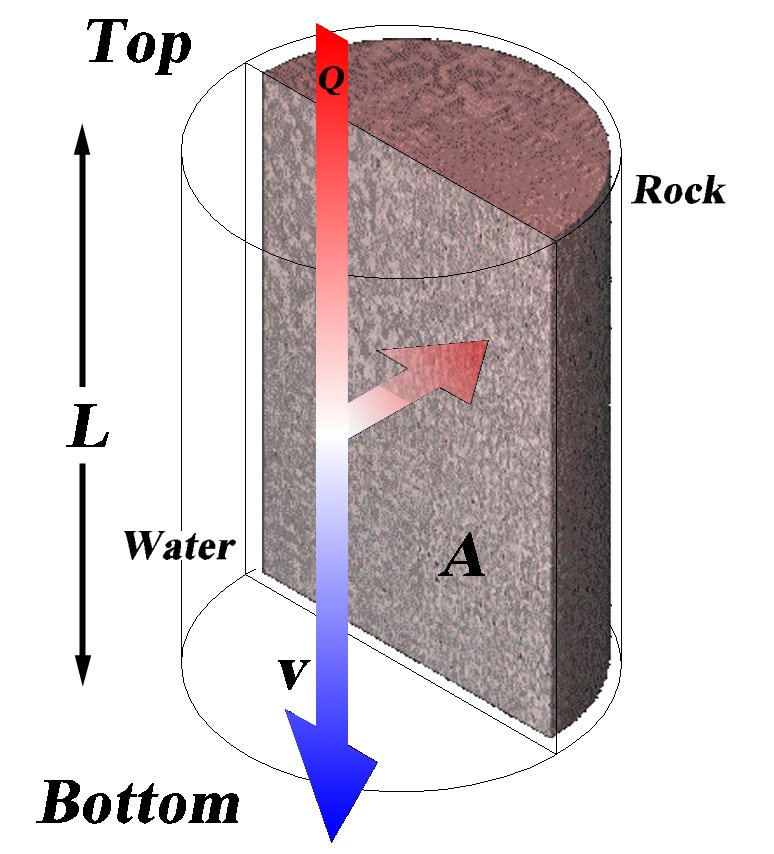
\includegraphics[scale=.25]{theorySlab.jpg}
\caption[Thermal Transfer Model]{\textbf{\emph{Thermal transfer inside the heat exchange vessel}} A simplified model of the gravitationally charged experimental sample vessel where heat is exchanged between a hydraulic flow (water) and a thermal sinking sample (rock - aggregate). This model, along with Fourier's Law, serves as the basis for the formulation of a cobble-level heat exchange model that draws its parametrization from data.\label{slab}}
\end{center}
\end{figure}

The method that follows is currently being developed by C.S. Thaxton as a means of providing a theoretical understanding of the heat exchange processes in aggregate materials. The work here is presented as a theoretical base that was derived from and ultimately supported by the data collected in this experimentation.

The experiment can be theorized in a general scenario that is founded on Fourier's Law, and does not depend on the sample or test material being of a un-consolidated nature. In this scenario, the test material is modeled as a solid slab for simplicity in determining a thermal contact area $A$ and in considering a flow regime. Furthermore, all heat transferred is assumed to take place only through a conduction mechanism, and convective or radiative processes are not considered in this formalism \citep{theoryKern}.

\noindent At any differential vertical segment $dl$, Fourier's Law is approximated as the following:
\begin{equation}\label{fouiers}
 \dot{Q}(L,t)=-\kappa A\;\frac{T(y,t)[W]-T(y,t)[R]}{R_{s}}
\end{equation}
Here, the aforementioned nomenclature holds, except instead of using a time-stepped temperature or energy value for numerical analysis, a differential is considered over both space and time, with $y$ representing a position along the sample's height. The gradient argument in Fourier's Law is assumed to be a finite distance between the water/rock interface and the center of the rock \citep{quench}. It is therefore represented by the rock's characteristic radius $R_{s}$. Solving this equation by means of variable separation and integration yields the following intermediate result.
\begin{equation}\label{Tbar}
\Delta Q_{net}=-\kappa\left(\dfrac{A}{R}\right) \int_{0}^{t_{f}} \left[ \dfrac{1}{L}\int_{0}^{L} T[WR](y,t)dy \right]dt\:=\:-\kappa\;\frac{A}{R}\int_{0}^{t_{f}}\bar{T}[WR](t)dt
\end{equation}
Where the bracketed term is the spatial average of $T(t)[WR]$ along $L$ and is numerically equivalent to Equation (\ref{rt}):
\begin{equation}\label{spatialT}
 \bar{T}(t)[WR]=\frac{1}{L}\int_{0}^{L}T(y,t)[WR]dL\;=\;\dfrac{-\Delta T(t)[TB]}{\sum\Delta T(t)[TB]}\left(2T[TOP]-T[AMBIENT]\right)
\end{equation}

By considering the first law of thermodynamics and net heat transfer as was discussed in the experiment section, it's possible to theoretically arrive at the following differential equation \citep{theoryKern}:
\begin{equation}\label{tempdiffeq}
 \dot{T}(y,t)[WR]=-\frac{\kappa(c_{R}-c_{W})}{C_{R}\;c_{W}}\frac{A}{R}\;T(y,t)[WR]
\end{equation}
This is soluble with the following function:
\begin{center}
\begin{equation}\label{solution}
\begin{aligned}
 T(y,t)[WR]=&T(y,0)[WR]e^{-\sigma_{f} t}\\
 \sigma_{f}=&-\frac{A(C_{R}-C_{W})}{R_{s}C_{W}}\;T_m\\
 T_m=&\frac{\kappa}{C_{R}}\\
\end{aligned}
\end{equation}
\end{center}
Equation (\ref{tempdiffeq}) can be simplified by letting $y=L$ and considering just the bulk temperature change over the entire sample and by assuming that the intial temperature difference between water and rock is equivalent to the total available potential difference between reservoir and ambient temperatures \citep{theoryKern}, let $T(0)[WR]=T_{o}$:
\begin{equation}\label{tempdiffeq2}
 \dot{T}(t)[WR]=T_{o}e^{-\sigma_{f} t}
\end{equation}

This solution is aligned with the result from the Thermal Potential Model. Understanding how various parameters in each of the respective exponents needs to be studied. The exponent in the Thermal Potential Model appears over simplified and the curve only matches well behaved or ideal energy transfers. The aforementioned empirical theory expands to include another exponential term that accounts for interaction area of the flow and rock, in addition to flow rate. 

The plots in Figure (\ref{steelHigh}) demonstrate that the empirical thermal model is directly consistent in predicting a vessel temperature differential by computing the temperature gradient as a function of length and time. However, more complex predictions fail to generate real values due to an inability to scale the flow and contact area parameters accurately. Because this supporting theory is still being developed, future research should seek to understand more exact parametrizations, especially with respect to flow and contact area.

This empirical model also introduces a second exponential term, consistent with a more general solution to the heat equation, and capable of accounting for flow related variables.
\begin{equation}\label{completetemp}
\begin{aligned}
\bar{T}[WR](y,t)=&\frac{1}{\beta L}T[WR](0,0)\;e^{-\alpha t}(1-e^{-\beta L})\\
\beta=&\left[\frac{C_{R}-C_{W}}{C_{R}\;C_{W}}\right]\;\frac{\kappa A}{\nu R_{s}}
\end{aligned}
\end{equation}


\begin{equation}\label{completeheat}
\begin{aligned}
Q_{net}=&Q_{0}-\frac{\gamma}{\alpha}(1-e^{-\alpha t})\\
\gamma=&\;\frac{\kappa A}{R_{s}}\frac{1}{\beta L}\;T[WR](0,0)(1-e^{-\beta L})
\end{aligned}
\end{equation}

\pagebreak

\begin{figure}[!h]
\begin{center}
\caption[Empirical Model and Data Comparison - Low]{\label{steelMed}}
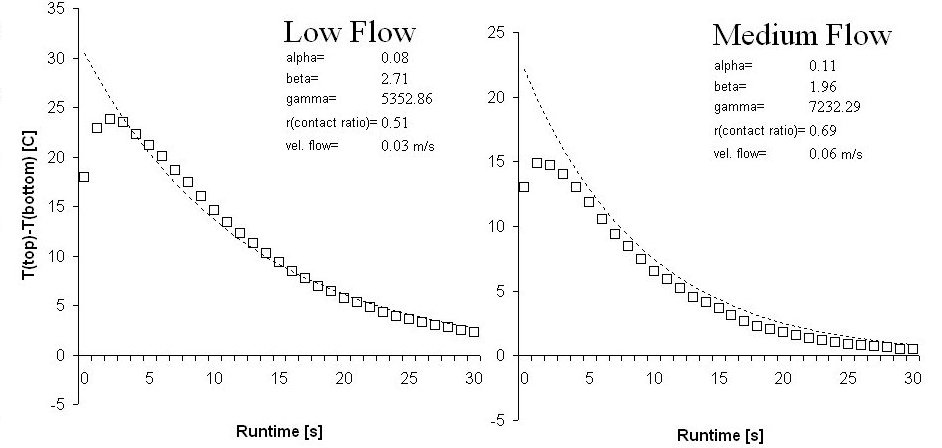
\includegraphics[scale=.5]{flowDouble.jpg}
\end{center}
\end{figure}

\begin{figure}[!h]
\begin{center}
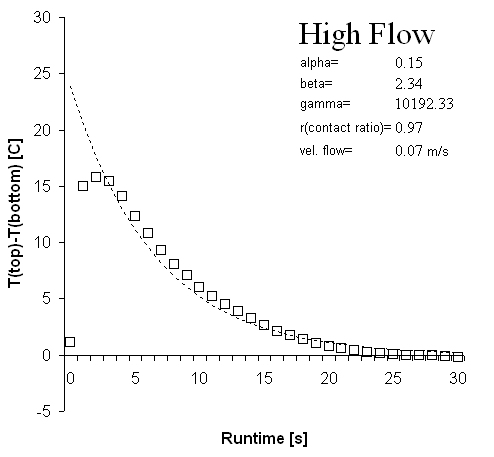
\includegraphics[scale=.5]{steelhighFlow.jpg}
\caption[Empirical Model and Data Comparison - High]{\textbf{\emph{Empirical model results vs. experimental temperature differences}} The empirically derived model successfully predicts the temperature difference across the vessel on a control sample of mild steel balls across a range of flows. The time and length dependent temperature gradient that defines the vessel heat exchange is part of this model. The flow rates are 0.25, 0.43 and 0.55 L/s, respectively.\label{steelHigh}}
\end{center}
\end{figure}
\pagebreak
